\hypertarget{i-dont-have-a-dream}{%
\section{I don't have a dream}\label{i-dont-have-a-dream}}

\begin{figure}[!ht]
  \begin{adjustwidth}{-\oddsidemargin-1in}{-\rightmargin}
    \centering
    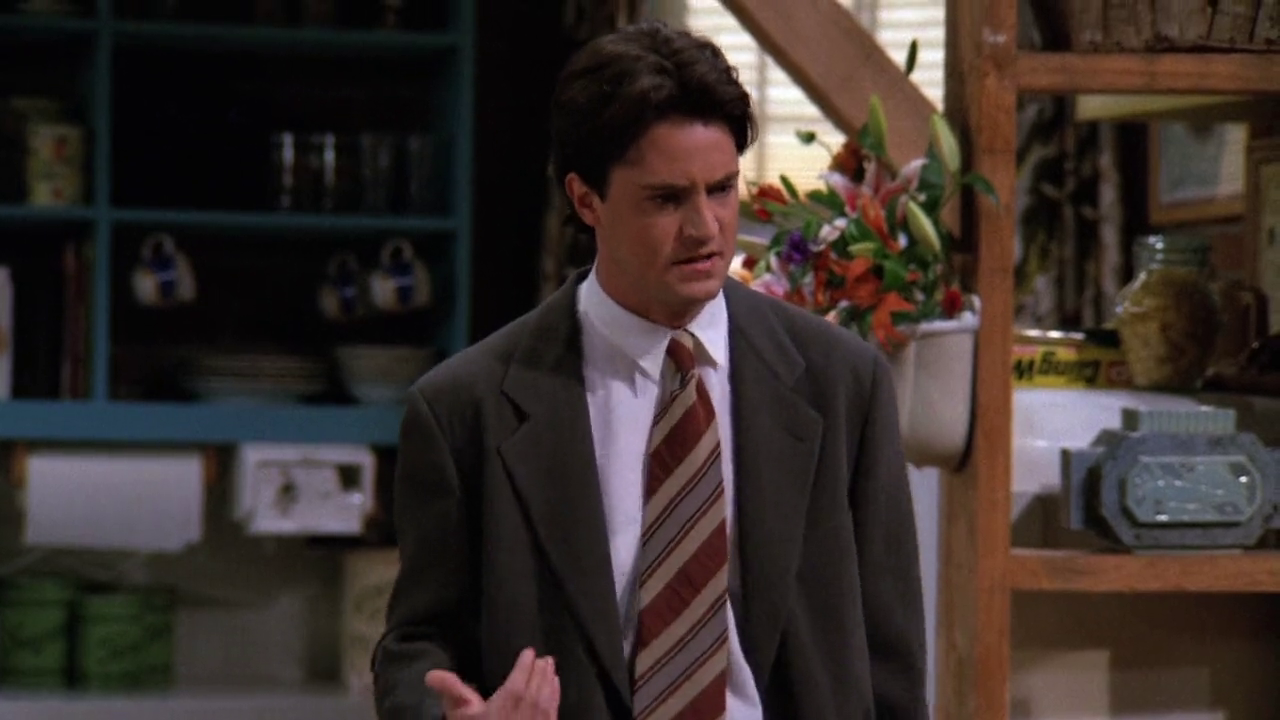
\includegraphics[trim={0 9cm 0 1cm,}, clip, width=\paperwidth]{./S01/img/15/i-don-t-have-a-dream.png}
    % \caption{I don’t have a dream\label{fig:i-don-t-have-a-dream}}
  \end{adjustwidth}
\end{figure}

\begin{tcolorbox}[enhanced,center upper,
    drop fuzzy shadow southeast, boxrule=0.3pt,
    lower separated=false, breakable,
    colframe=black!30!dialogoBorder,colback=white]
\begin{minipage}[c]{0.16\linewidth}
  \raisebox{\dimexpr-\height+\ht\strutbox\relax}{
    \centering 
\includegraphics[width=1.4cm]{./assets/img/chandler.png}
  }
   & \centering \scriptsize{Chandler}
\end{minipage}
\hfill
\begin{minipage}[c]{0.8\linewidth}
  \textbf{- I don't have a dream.}\\
  - Eu não tenho um sonho.
\end{minipage}

\medskip
\begin{minipage}[c]{0.16\linewidth}
  \raisebox{\dimexpr-\height+\ht\strutbox\relax}{
    \centering 
\includegraphics[width=1.4cm]{./assets/img/ross.png}
  }
   & \centering \scriptsize{Ross}
\end{minipage}
\hfill
\begin{minipage}[c]{0.8\linewidth}
  \textbf{- Ah, the lesser known I Don't Have a Dream speech.}\\
  - Esse discurso é menos conhecido.
\end{minipage}
\end{tcolorbox}

\saveparinfos
\noindent
\begin{minipage}[c]{0.5\textwidth}\useparinfo

Ross faz um trocadilho com o discurso de \emph{Martin Luther King Jr.}
(1929-1968) \emph{I have a dream}, \emph{Eu tenho um sonho} em
português. O discurso vocalizado em 28 de Agosto de 1963 pedia igualdade
para o povo negro americano.\footnote{\sloppy ProJuris - Discurso de Martin Luther King Jr.. \url{https://bit.ly/3lioimk}}
\footnote{\sloppy Martin Luther King Jr. - Discurso com legendas - YouTube. \url{https://www.youtube.com/watch?v=fz_7luovxPc}}

\end{minipage}\hfill
\begin{minipage}[c]{0.5\textwidth}

\begin{figure}
  \centering
  \begin{tikzpicture}
    \node [inner sep=0pt] at (0,0) {
      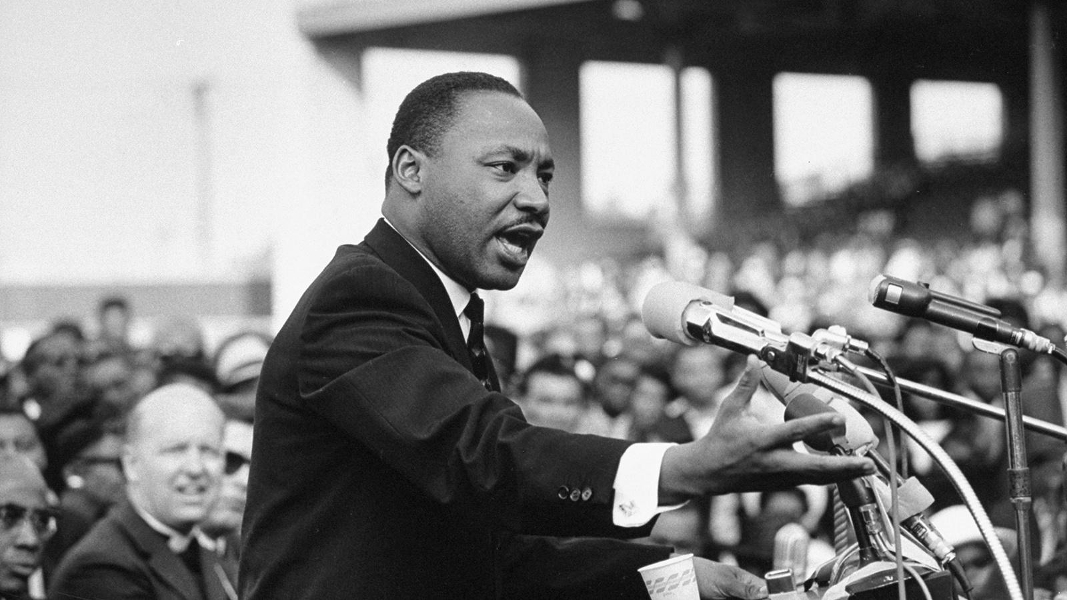
\includegraphics[width=0.8\textwidth,keepaspectratio]{./S01/img/15/martin-luther-king-jr.jpg}
    };
    \draw [white, rounded corners=\ClipSep, line width=\ClipSep]
    (current bounding box.north west) --
    (current bounding box.north east) --
    (current bounding box.south east) --
    (current bounding box.south west) -- cycle
    ;
    \end{tikzpicture}
    \caption{Martin Luther King Jr.\label{fig:martin-luther-king-jr}}
\end{figure}

\end{minipage}

\hypertarget{brians-song}{%
\section{Brian's Song}\label{brians-song}}

\begin{figure}[!ht]
  \begin{adjustwidth}{-\oddsidemargin-1in}{-\rightmargin}
    \centering
    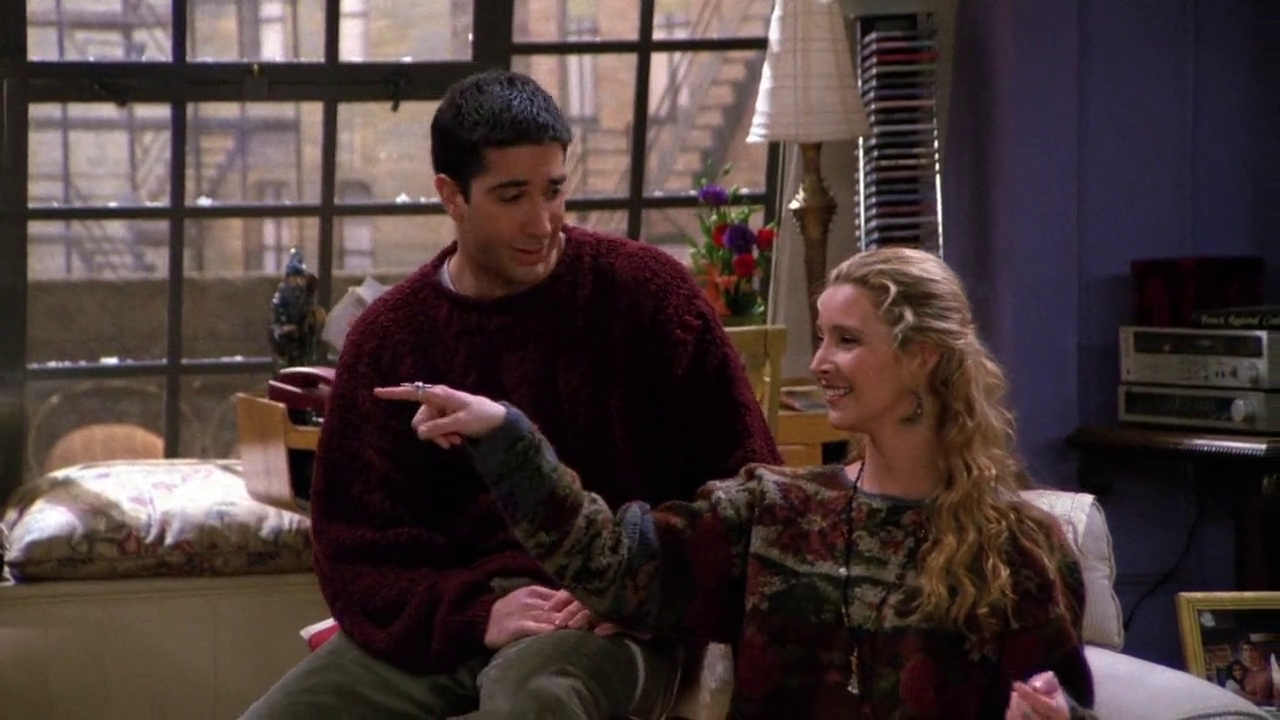
\includegraphics[trim={0 7cm 0 2cm,}, clip, width=\paperwidth]{./S01/img/15/brian-s-song.png}
    % \caption{Brian’s Song\label{fig:brian-s-song}}
  \end{adjustwidth}
\end{figure}

\begin{tcolorbox}[enhanced,center upper,
    drop fuzzy shadow southeast, boxrule=0.3pt,
    lower separated=false,
    colframe=black!30!dialogoBorder,colback=white]
\begin{minipage}[c]{0.16\linewidth}
  \raisebox{\dimexpr-\height+\ht\strutbox\relax}{
    \centering 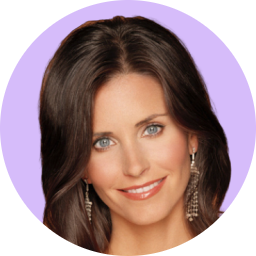
\includegraphics[width=1.4cm]{./assets/img/monica.png}
  }
   & \centering \scriptsize{Monica}
\end{minipage}
\hfill
\begin{minipage}[c]{0.8\linewidth}
  \textbf{- Oh, I love my life. I love my life.}\\
  - Eu adoro a minha vida!
\end{minipage}

\medskip
\begin{minipage}[c]{0.16\linewidth}
  \raisebox{\dimexpr-\height+\ht\strutbox\relax}{
    \centering 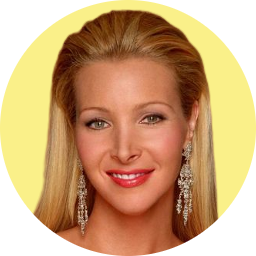
\includegraphics[width=1.4cm]{./assets/img/phoebe.png}
  }
   & \centering \scriptsize{Phoebe}
\end{minipage}
\hfill
\begin{minipage}[c]{0.8\linewidth}
  \textbf{- Brian's Song.}\\
  - Brian's Song.
\end{minipage}
\end{tcolorbox}

Enquanto Monica entra no apartamento alegre por ter tido uma boa
entrevista, Phoebe acha que a fala dela é uma referência ao filme
\emph{Brian's Song} (1971), que conta a histório de \emph{Brian
Piccolo}, um atleta de futebol americano que descobre um câncer terminal
logo que entra para o time profissional.\footnote{\sloppy Brian’s Song - TMDB. \url{https://www.themoviedb.org/movie/18047-brian-s-song}}

Isso, certamente, remete ao fato de que sua mãe evitava que ela
assistisse ao final de filmes trágicos, como mais tarde seria revelado
em
\textbf{\textcolor{primarycolor}{S02E20 - Aquele em que o velho Yeller morre}}.

\begin{figure}
  \centering
  \begin{tikzpicture}
    \node [inner sep=0pt] at (0,0) {
      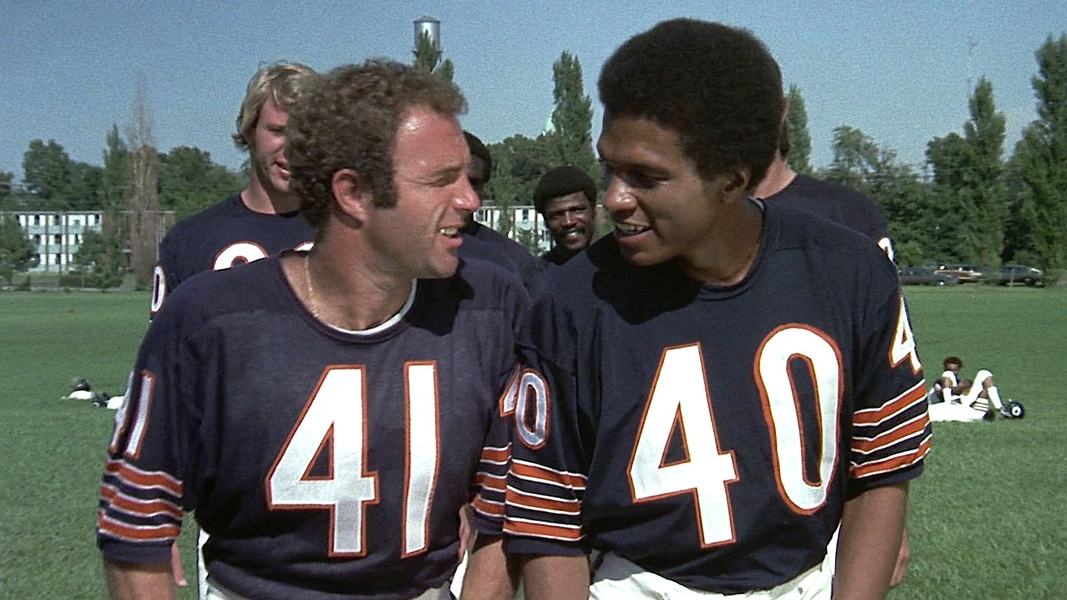
\includegraphics[width=0.8\textwidth,keepaspectratio]{./S01/img/15/brian-s-song-movie.jpg}
    };
    \draw [white, rounded corners=\ClipSep, line width=\ClipSep]
    (current bounding box.north west) --
    (current bounding box.north east) --
    (current bounding box.south east) --
    (current bounding box.south west) -- cycle
    ;
    \end{tikzpicture}
    \caption{Brian’s Song - Filme\label{fig:brian-s-song-filme}}
\end{figure}

\hypertarget{a-blond-woman-and-some-bears}{%
\section{A blond woman and some
bears}\label{a-blond-woman-and-some-bears}}

\begin{figure}[!ht]
  \begin{adjustwidth}{-\oddsidemargin-1in}{-\rightmargin}
    \centering
    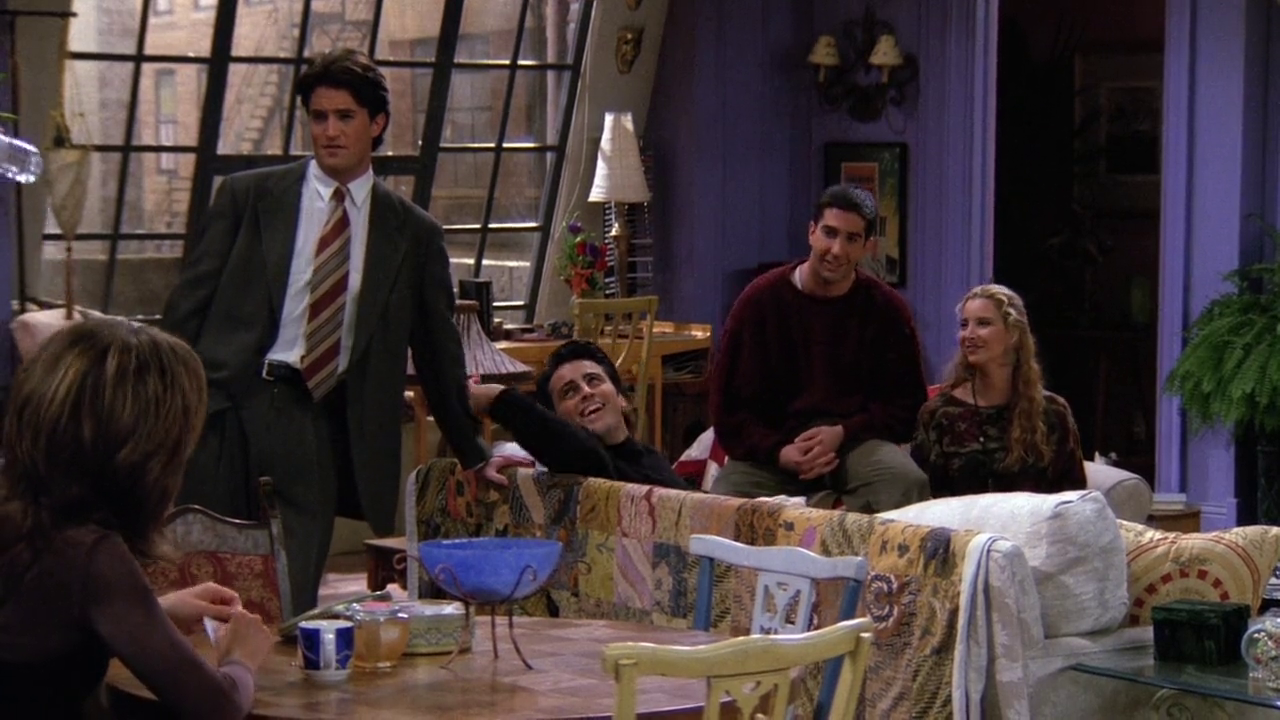
\includegraphics[trim={0 9cm 0 1cm,}, clip, width=\paperwidth]{./S01/img/15/a-blond-woman-and-some-bears.png}
    % \caption{A blond woman and some bears\label{fig:a-blond-woman-and-some-bears}}
  \end{adjustwidth}
\end{figure}

\begin{tcolorbox}[enhanced,center upper,
    drop fuzzy shadow southeast, boxrule=0.3pt,
    lower separated=false, breakable,
    colframe=black!30!dialogoBorder,colback=white]
\begin{minipage}[c]{0.16\linewidth}
  \raisebox{\dimexpr-\height+\ht\strutbox\relax}{
    \centering 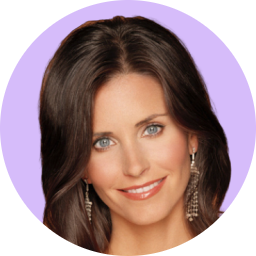
\includegraphics[width=1.4cm]{./assets/img/monica.png}
  }
   & \centering \scriptsize{Monica}
\end{minipage}
\hfill
\begin{minipage}[c]{0.8\linewidth}
  \textbf{- It's not too big, not too small. It's just right.}\\
  - Não é nem grande nem pequeno, é perfeito.
\end{minipage}

\medskip
\begin{minipage}[c]{0.16\linewidth}
  \raisebox{\dimexpr-\height+\ht\strutbox\relax}{
    \centering 
\includegraphics[width=1.4cm]{./assets/img/chandler.png}
  }
   & \centering \scriptsize{Chandler}
\end{minipage}
\hfill
\begin{minipage}[c]{0.8\linewidth}
  \textbf{- Was it formerly owned by a blond woman and some bears?}\\
  - A antiga dona era loira e tinha ursos?
\end{minipage}
\end{tcolorbox}

Depois de Monica explicar como era o restaurante que ela poderia
trabalhar caso passasse na entrevista, Chandler menciona uma antiga dona
loira e uns ursos. Ele faz referência ao conto \emph{The Story of the
Three Bears} (1837) de \emph{Robert Southey} (1744-1843)\footnote{\sloppy Robert Southey - Encyclopædia Britannica. \url{https://www.britannica.com/biography/Robert-Southey}},
no qual há uma paráfrase do diálogo de Monica com o livro.\footnote{\sloppy The Story of the Three Bears na American Literature (Inglês). \url{https://americanliterature.com/childrens-stories/goldilocks-and-the-three-bears}}
No Brasil a história ficou conhecida como \emph{Cachinhos Dourados e os
Três Ursos}.

Para dar um exemplo, o texto conta como \emph{Cachinhos Dourados}
experimentou o mingau do Papai Urso e achou quente, depois experimentou
o da Mamãe Urso e achou frio, e, por fim, experimentou o mingau do
Pequeno Urso, e ele nem estava quente nem frio, estava
perfeito.\footnote{Batten, Cundall, Lang. \emph{Goldilocks and the Three
  Bears: Special Edition}. John Batten 2014.}

\hypertarget{innsbruck}{%
\section{Innsbruck}\label{innsbruck}}

\begin{figure}[!ht]
  \begin{adjustwidth}{-\oddsidemargin-1in}{-\rightmargin}
    \centering
    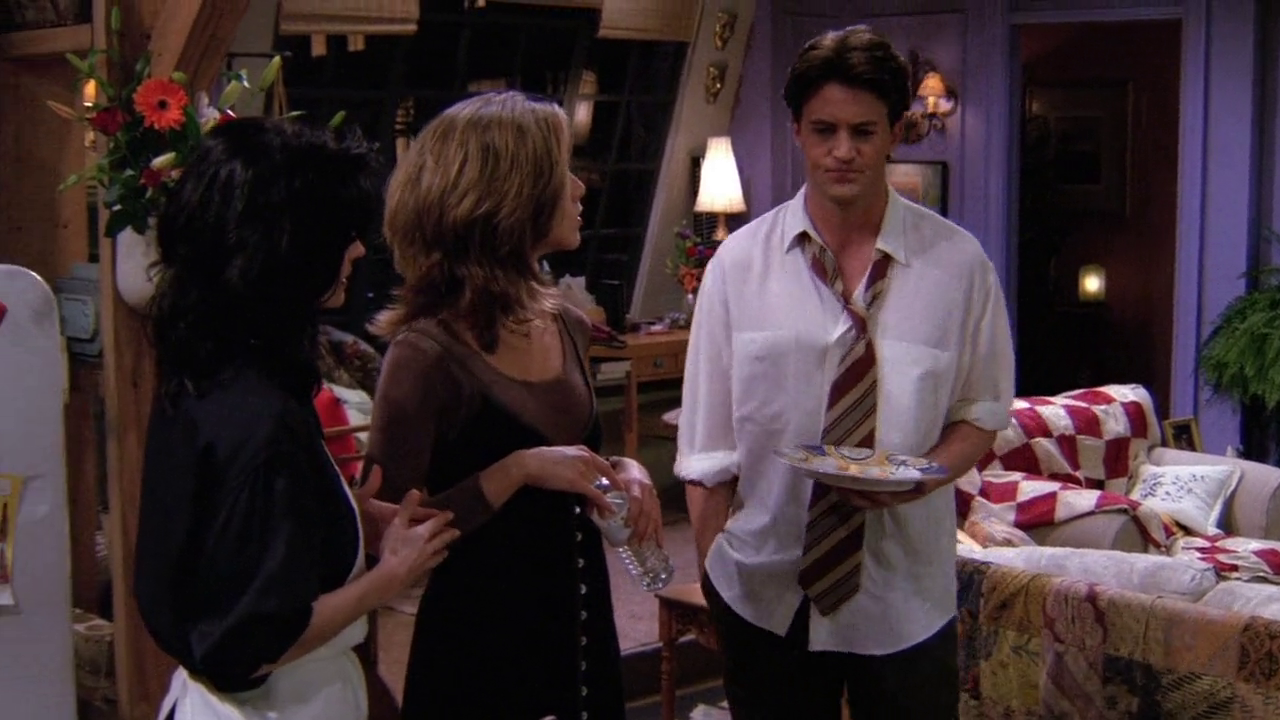
\includegraphics[trim={0 8cm 0 0cm,}, clip, width=\paperwidth]{./S01/img/15/innsbruck.png}
    % \caption{Innsbruck\label{fig:innsbruck}}
  \end{adjustwidth}
\end{figure}

\begin{tcolorbox}[enhanced,center upper,
    drop fuzzy shadow southeast, boxrule=0.3pt,
    lower separated=false, breakable,
    colframe=black!30!dialogoBorder,colback=white]
\begin{minipage}[c]{0.16\linewidth}
  \raisebox{\dimexpr-\height+\ht\strutbox\relax}{
    \centering 
\includegraphics[width=1.4cm]{./assets/img/rachel.png}
  }
   & \centering \scriptsize{Rachel}
\end{minipage}
\hfill
\begin{minipage}[c]{0.8\linewidth}
  \textbf{- [...] And I've sort of been maintaining my amateur status so that I can waitress in the Olympics.}\\
  - [...] E eu continuo sendo amadora para poder competir nas Olimpíadas.
\end{minipage}

\medskip
\begin{minipage}[c]{0.16\linewidth}
  \raisebox{\dimexpr-\height+\ht\strutbox\relax}{
    \centering 
\includegraphics[width=1.4cm]{./assets/img/chandler.png}
  }
   & \centering \scriptsize{Chandler}
\end{minipage}
\hfill
\begin{minipage}[c]{0.8\linewidth}
  \textbf{- You know, I don't mean to brag, but I waited tables at Innsbruck in '76. Amuse-bouche?}\\
  - Não quero me gabar, mas fui garçom em Innsbruck, em '76. Amuse-bouche?
\end{minipage}
\end{tcolorbox}

Chandler faz pouco da Rachel e insinua que foi garçom em
\emph{Innsbruck} em '76. Ele se refere aos \emph{Jogos Olímpicos de
Inverno} (1976), ocorridos na cidade de \emph{Innsbruck}, na Áustria. Os
jogos ocorreram entre os dias 4 e 15 de Fevereiro com representantes de
37 países. O Brasil não participou.\footnote{\sloppy Innsbruck 176 - Página oficial (Inglês). \url{https://www.olympic.org/innsbruck-1976}}

\hypertarget{cheech}{%
\section{Cheech}\label{cheech}}

\begin{figure}[!ht]
  \begin{adjustwidth}{-\oddsidemargin-1in}{-\rightmargin}
    \centering
    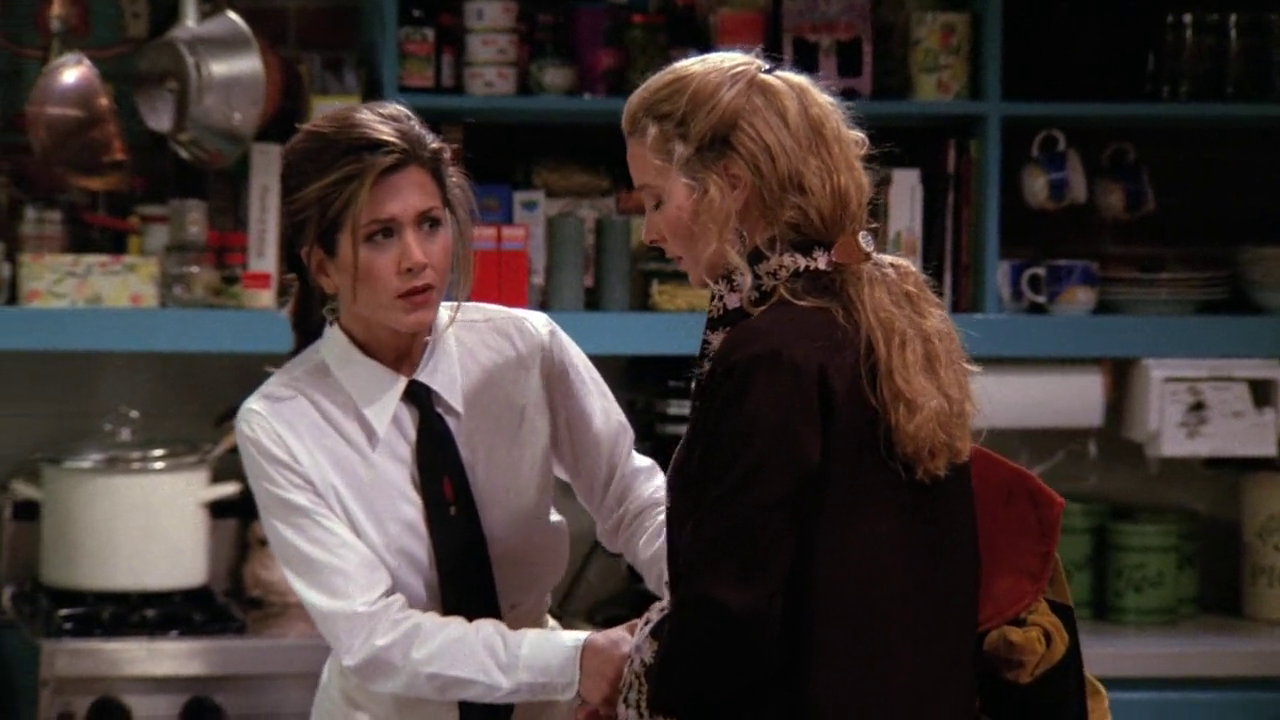
\includegraphics[trim={0 9cm 0 1cm,}, clip, width=\paperwidth]{./S01/img/15/cheech.png}
    % \caption{Cheech\label{fig:cheech}}
  \end{adjustwidth}
\end{figure}

\begin{tcolorbox}[enhanced,center upper,
    drop fuzzy shadow southeast, boxrule=0.3pt,
    lower separated=false, breakable,
    colframe=black!30!dialogoBorder,colback=white]
\begin{minipage}[c]{0.16\linewidth}
  \raisebox{\dimexpr-\height+\ht\strutbox\relax}{
    \centering 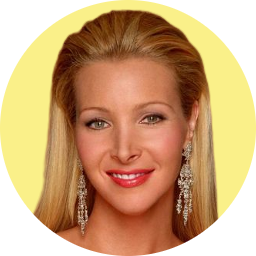
\includegraphics[width=1.4cm]{./assets/img/phoebe.png}
  }
   & \centering \scriptsize{Phoebe}
\end{minipage}
\hfill
\begin{minipage}[c]{0.8\linewidth}
  \textbf{- Smoked a joint, you know? Lit a bone. Weed, hemp, ganja.}\\
  - Fumou um baseado, maconha, erva, hemp.
\end{minipage}

\medskip
\begin{minipage}[c]{0.16\linewidth}
  \raisebox{\dimexpr-\height+\ht\strutbox\relax}{
    \centering 
\includegraphics[width=1.4cm]{./assets/img/rachel.png}
  }
   & \centering \scriptsize{Rachel}
\end{minipage}
\hfill
\begin{minipage}[c]{0.8\linewidth}
  \textbf{- Okay, I'm with you, Cheech.}\\
  - Já entendi, Cheech.
\end{minipage}
\end{tcolorbox}

Phoebe conta a Rachel que Steve, o dono do restaurante, havia dado um
``tapa'' no caminho até o apartamento. Percebendo que Rachel não havia
entendido bem, Phoebe menciona vários sinônimos para maconha, até que
Rachel a interrompe e menciona \emph{Cheech}. \emph{Richard ``Cheech''
Marin} junto com \emph{Tommy Chong} formam a dupla de comédia
\emph{Cheech \& Chong} (1971). Eles se apresentavam em
\emph{stand-up's}, gravaram discos e filmes baseados na era
\emph{hippie}.\footnote{\sloppy Cheech \& Chong - Wikipédia. \url{https://bit.ly/3qbBZY0}}

Abaixo uma cena do filme \emph{Up in Smoke} (1978), \emph{Cheech} à
direita e \emph{Chong} à esquerda.

\begin{figure}
  \centering
  \begin{tikzpicture}
    \node [inner sep=0pt] at (0,0) {
      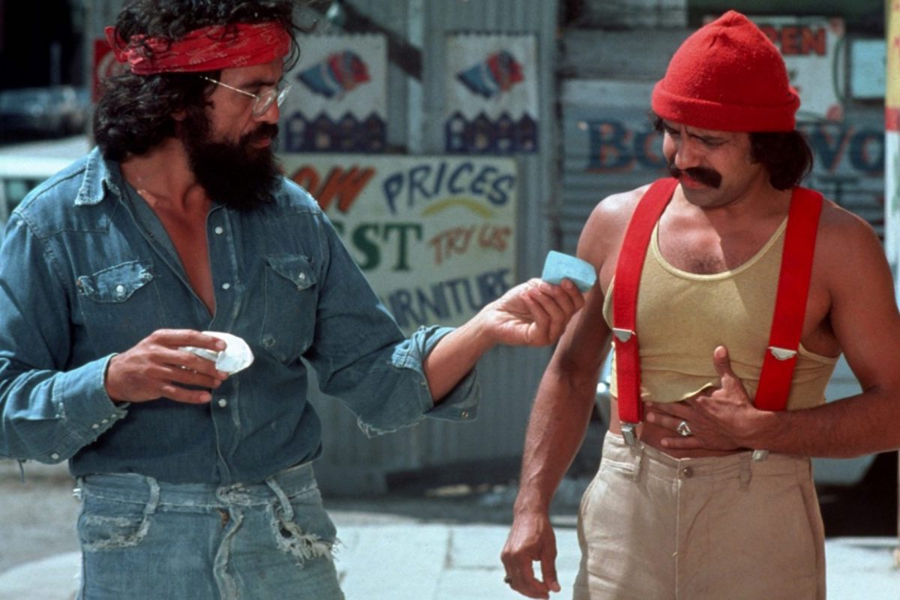
\includegraphics[width=0.6\textwidth,keepaspectratio]{./S01/img/15/up-in-smoke.jpg}
    };
    \draw [white, rounded corners=\ClipSep, line width=\ClipSep]
    (current bounding box.north west) --
    (current bounding box.north east) --
    (current bounding box.south east) --
    (current bounding box.south west) -- cycle
    ;
    \end{tikzpicture}
    \caption{Up in Smoke\label{fig:up-in-smoke}}
\end{figure}

\hypertarget{james-michener}{%
\section{James Michener}\label{james-michener}}

\begin{figure}[!ht]
  \begin{adjustwidth}{-\oddsidemargin-1in}{-\rightmargin}
    \centering
    
\includegraphics[trim={0 9cm 0 2cm,}, clip, width=\paperwidth]{./S01/img/15/james-michener.png}
    % \caption{James Michener\label{fig:james-michener}}
  \end{adjustwidth}
\end{figure}

\begin{tcolorbox}[enhanced,center upper,
    drop fuzzy shadow southeast, boxrule=0.3pt,
    lower separated=false, breakable,
    colframe=black!30!dialogoBorder,colback=white]
\begin{minipage}[c]{0.16\linewidth}
  \raisebox{\dimexpr-\height+\ht\strutbox\relax}{
    \centering 
\includegraphics[width=1.4cm]{./assets/img/joey.png}
  }
   & \centering \scriptsize{Joey}
\end{minipage}
\hfill
\begin{minipage}[c]{0.8\linewidth}
  \textbf{- So, uh, how did it go with Celia?}\\
  - Então, como foi com Celia?
\end{minipage}

\medskip
\begin{minipage}[c]{0.16\linewidth}
  \raisebox{\dimexpr-\height+\ht\strutbox\relax}{
    \centering 
\includegraphics[width=1.4cm]{./assets/img/ross.png}
  }
   & \centering \scriptsize{Ross}
\end{minipage}
\hfill
\begin{minipage}[c]{0.8\linewidth}
  \textbf{- I was unbelievable.}\\
  - Eu fui inacreditável.
\end{minipage}

\medskip
\begin{minipage}[c]{0.16\linewidth}
  \raisebox{\dimexpr-\height+\ht\strutbox\relax}{
    \centering 
\includegraphics[width=1.4cm]{./assets/img/joey.png}
  }
   & \centering \scriptsize{Joey}
\end{minipage}
\hfill
\begin{minipage}[c]{0.8\linewidth}
  \textbf{- All right, Ross.}\\
  - É isso aí, Ross.
\end{minipage}

\medskip
\begin{minipage}[c]{0.16\linewidth}
  \raisebox{\dimexpr-\height+\ht\strutbox\relax}{
    \centering 
\includegraphics[width=1.4cm]{./assets/img/ross.png}
  }
   & \centering \scriptsize{Ross}
\end{minipage}
\hfill
\begin{minipage}[c]{0.8\linewidth}
  \textbf{- I was the James Michener of dirty talk.}\\
  - Fui o James Michener da sacanagem.
\end{minipage}
\end{tcolorbox}

\saveparinfos
\noindent
\begin{minipage}[c]{0.5\textwidth}\useparinfo

Descrevendo seu encontro com Celia, Ross menciona \emph{James Michener}
(1907-1997), autor norte-americano conhecido por seus romances extensos
devido a detalhadas descrições, tanto geográficas, familiares e
históricas. Ele às vezes levava anos na preparação de seus livros, como
por exemplo em \emph{Spain for Iberia: Spanish Travels and Reflections}
(1968).\footnote{\sloppy James Michener - Encyclopædia Britannica (Inglês). \url{https://www.britannica.com/biography/James-Albert-Michener}}

\end{minipage}\hfill
\begin{minipage}[c]{0.5\textwidth}

\begin{figure}
  \centering
  \begin{tikzpicture}
    \node [inner sep=0pt] at (0,0) {
      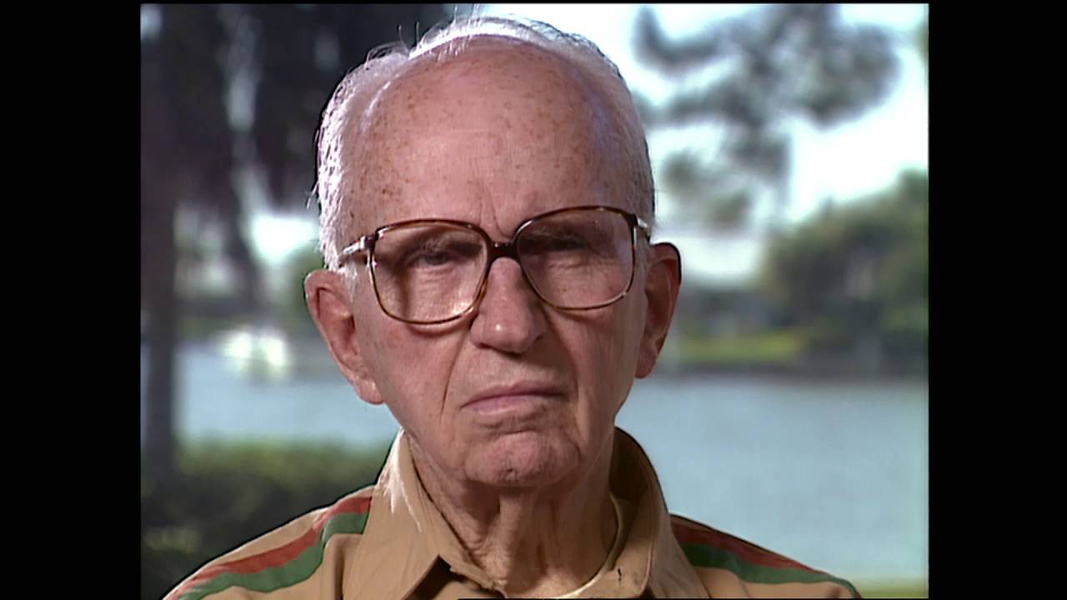
\includegraphics[width=0.8\textwidth,keepaspectratio]{./S01/img/15/james-michener-foto.jpg}
    };
    \draw [white, rounded corners=\ClipSep, line width=\ClipSep]
    (current bounding box.north west) --
    (current bounding box.north east) --
    (current bounding box.south east) --
    (current bounding box.south west) -- cycle
    ;
    \end{tikzpicture}
    \caption{James Michener - Foto\label{fig:james-michener-foto}}
\end{figure}

\end{minipage}
